\documentclass[12pt,a4paper]{article}
\usepackage[left=2cm,right=2cm,top=2cm,bottom=2cm]{geometry}
\usepackage[utf8]{inputenc}
\usepackage[T2A]{fontenc}
\usepackage{amsmath}
\usepackage{amssymb}
\usepackage{graphicx}
\usepackage[russian]{babel}
\usepackage{indentfirst}
\usepackage{listings}
\usepackage{xcolor}
\usepackage{subcaption}
\usepackage{hyperref}

\hypersetup{
  colorlinks=true,
  urlcolor= blue,
  citecolor=blue,
  linkcolor= blue,
}

\title{Отчет по лабораторной работе по дисциплине "Математическая статистика"}
\author{Скворцов Владимир Сергеевич (5030102/10201)}
\date{\today}

\begin{document}

	\begin{titlepage}

		\Large

		\begin{center}
			Санкт-Петербургский \\ Политехнический университет Петра Великого

			\vspace{10em}

			\textbf{Отчет по лабораторной работе} \\
			\textbf{по дисциплине}\\
			"\textbf{Математическая статистика}"

			\vspace{2em}

		\end{center}

		\vspace{6em}

		\newbox{\lbox}
		\savebox{\lbox}{\hbox{Табакова Виктория Олеговна}}
		\newlength{\maxl}
		\setlength{\maxl}{\wd\lbox}
		\hfill\parbox{12cm}{
			\hspace*{3cm}\hspace*{-5cm}Студент:\hfill\hbox to\maxl{Табакова Виктория Олеговна\hfill}\\
			\hspace*{3cm}\hspace*{-5cm}Преподаватель:\hfill\hbox to\maxl{Васильчук Владимир Юрьевич}\\
			\\
			\hspace*{3cm}\hspace*{-5cm}Группа:\hfill\hbox to\maxl{5030102/10401}\\
		}

		\vspace{\fill}

		\begin{center}
			Санкт-Петербург \\ 2024
		\end{center}

	\end{titlepage}

	\tableofcontents\newpage

	\section{Постановка задачи}

	Имеется выборка некоторой СВ \( \xi \) в виде интервального статистического ряда (табл.). Требуется:

	\begin{enumerate}
		\item Построить гистограмму и график эпмирической функции распределения \( F_n(x) \);
		\item Вычислить выборочные: среднее, дисперсию, медиану, коэффициент вариации, коэффициент ассиметрии, эксцесс;
		\item Добавить искусственно к данным большую флуктуацию (порядка 1000). Как изменятся вычисленные параметры? Почему?
	\end{enumerate}

	\begin{enumerate}
		\item \

		\begin{table}[htbp!]
			\centering
			\begin{tabular}{ |c|c|c|c|c|c| }
				\hline
				Интервал & (21; 23) & (23; 25) & (25; 27) & (27; 29) & (29; 31) \\
				\hline
				Частота & 30 & 70 & 65 & 30 & 5 \\
				\hline
			\end{tabular}
		\end{table}

		\vspace{4em}

		\item \

		\begin{table}[htbp!]
			\centering
			\begin{tabular}{ |c|c|c|c|c|c| }
				\hline
				Интервал & (40; 45) & (45; 50) & (50; 55) & (55; 60) & (60; 60) \\
				\hline
				Частота & 50 & 100 & 105 & 40 & 5 \\
				\hline
			\end{tabular}
		\end{table}

		\vspace{4em}

		\item \

		\begin{table}[htbp!]
			\centering
			\begin{tabular}{ |c|c|c|c|c|c| }
				\hline
				Интервал & (100; 105) & (105; 110) & (110; 115) & (115; 120) & (120; 125) \\
				\hline
				Частота & 45 & 105 & 100 & 40 & 10 \\
				\hline
			\end{tabular}
		\end{table}

		\vspace{4em}

		\item \

		\begin{table}[htbp!]
			\centering
			\begin{tabular}{ |c|c|c|c|c|c| }
				\hline
				Интервал & (10; 15) & (15; 20) & (20; 25) & (25; 30) & (30; 35) \\
				\hline
				Частота & 60 & 140 & 135 & 55 & 10 \\
				\hline
			\end{tabular}
		\end{table}

		\vspace{4em}

		\item \

		\begin{table}[htbp!]
			\centering
			\begin{tabular}{ |c|c|c|c|c|c| }
				\hline
				Интервал & (80; 90) & (90; 100) & (100; 110) & (110; 120) & (120; 130) \\
				\hline
				Частота & 80 & 165 & 170 & 65 & 20 \\
				\hline
			\end{tabular}
		\end{table}

		\vspace{4em}

		\item \

		\begin{table}[htbp!]
			\centering
			\begin{tabular}{ |c|c|c|c|c|c| }
				\hline
				Интервал & (140; 145) & (145; 150) & (150; 155) & (155; 160) & (160; 165) \\
				\hline
				Частота & 60 & 140 & 135 & 55 & 10 \\
				\hline
			\end{tabular}
		\end{table}

		\vspace{4em}

		\item \

		\begin{table}[htbp!]
			\centering
			\begin{tabular}{ |c|c|c|c|c|c| }
				\hline
				Интервал & (170; 185) & (185; 200) & (200; 215) & (215; 230) & (230; 245) \\
				\hline
				Частота & 80 & 165 & 170 & 65 & 20 \\
				\hline
			\end{tabular}
		\end{table}

		\vspace{4em}

		\item \

		\begin{table}[htbp!]
			\centering
			\begin{tabular}{ |c|c|c|c|c|c| }
				\hline
				Интервал & (490; 495) & (495; 500) & (500; 505) & (505; 510) & (510; 515) \\
				\hline
				Частота & 110 & 240 & 235 & 95 & 20 \\
				\hline
			\end{tabular}
		\end{table}

		\vspace{4em}

		\item \

		\begin{table}[htbp!]
			\centering
			\begin{tabular}{ |c|c|c|c|c|c| }
				\hline
				Интервал & (130; 150) & (150; 170) & (170; 190) & (190; 210) & (210; 230) \\
				\hline
				Частота & 95 & 200 & 205 & 80 & 20 \\
				\hline
			\end{tabular}
		\end{table}

		\vspace{4em}

		\item \

		\begin{table}[htbp!]
			\centering
			\begin{tabular}{ |c|c|c|c|c|c| }
				\hline
				Интервал & (150; 175) & (175; 200) & (200; 225) & (225; 250) & (250; 275) \\
				\hline
				Частота & 110 & 240 & 235 & 95 & 20 \\
				\hline
			\end{tabular}
		\end{table}

		\vspace{4em}
	\end{enumerate}


	\section{Теоретическое обоснование}

	\begin{itemize}
		\item Выборочное среднее

		\begin{equation} \label{eq:mean}
			\overline{x} = \tfrac{1}{n}\sum_{i = 1}^{n}x_i
		\end{equation}

		\item Выборочная медиана

		\begin{equation} \label{eq:median}
			med\ x = \left\{
			\begin{array}{ccl}
			x_{(l + 1)} & \text{при} & n = 2l + 1\\
			\dfrac{x_{(l)} + x_{(l + 1)}}{2} & \text{при} & n = 2l
			\end{array}
			\right.
		\end{equation}

		\item Выборочная дисперсия

		\begin{equation} \label{eq:dispersion}
			D(z) = \overline{z^2} - \overline{z}^2
		\end{equation}

		\item Выборочное стандартное отклонение

		\begin{equation}
			\sigma = \sqrt{\frac{\sum (x_i - \bar x)^2}{n - 1}}
		\end{equation}

		\item Выборочный коэффициент вариации

		\begin{equation}
			CV = \sigma / \bar x
		\end{equation}

		\item Выборочный коэффициент ассиметии

		\begin{equation}
			A = \frac{n}{(n-1)(n-2)} \times \Sigma \left(\frac{(x_i - \bar x)}{\sigma}\right)^3
		\end{equation}

		\item Выборочный эксцесс

		\begin{equation}
			E = \frac{n(n + 1)}{(n-1)(n-2)(n-3)} \times \Sigma \left(\frac{(x_i - \mu)}{\sigma}\right)^4 - \frac{3(n - 1)^2}{(n - 2)(n - 3)}
		\end{equation}
	\end{itemize}

	\section{Описание работы}
	Лабораторные работы выполнены с использованием Python и его сторонних библиотек \verb!numpy!, \verb!pandas!, \verb!matplotlib!.

	Ссылка на GitHub репозиторий: \href{https://github.com/VictoriaTabakova/mathematical-statics}{https://github.com/VictoriaTabakova/mathematical-statics}

	\newpage

	\section{Результаты}

	\begin{figure}[htbp!]
		\begin{subfigure}[htbp!]{0.8\textwidth}
			\begin{center}
				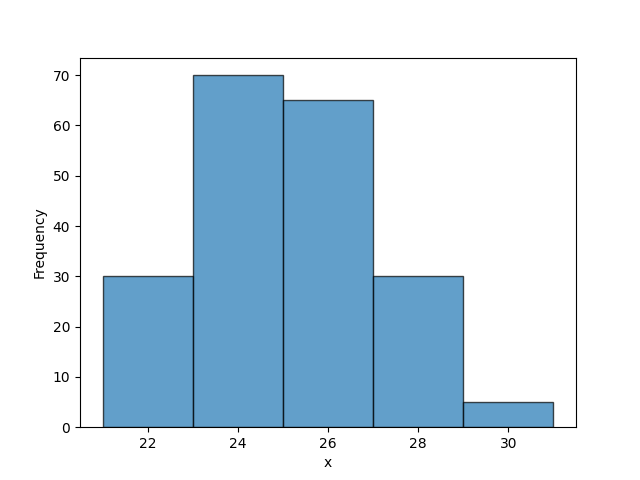
\includegraphics[width = 0.8\linewidth]{../graphics/1_hist.png}
				\caption{Гистограмма}
			\end{center}
		\end{subfigure}

		\begin{subfigure}[htbp!]{0.8\textwidth}
			\begin{center}
				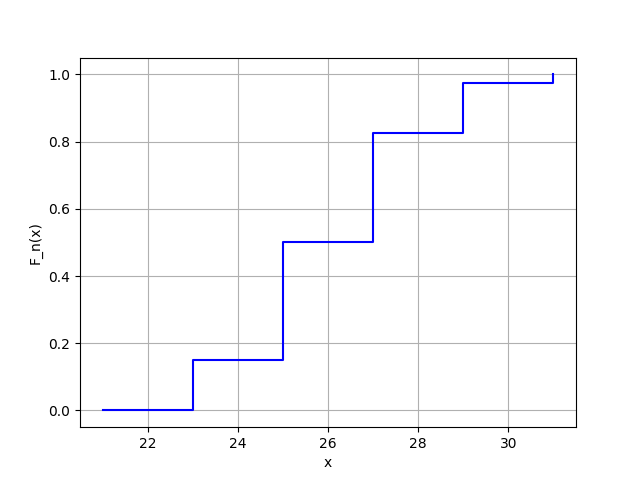
\includegraphics[width = 0.8\linewidth]{../graphics/1_cdf.png}
				\caption{Эмпирическая функция распределения}
			\end{center}
		\end{subfigure}

		\begin{subtable}[htbp!]{0.8\textwidth}
			\centering
			\begin{tabular}{ |c|c|c|c|c|c|c| }
				\hline
				& \( \bar x \) & \( med x \) & \( D(x) \) & \( CV \) & \( A \) & \( E \) \\
				\hline
				Без флактуаций & 25.1 & 25.0 & 3.99 & 0.08 & 0.24 & -0.51 \\
				\hline
				С флактуациями & 837.52 & 1000.0 & 132004.83 & 0.43 & -1.79 & 1.2 \\
				\hline
			\end{tabular}
		\end{subtable}
	\end{figure}

	\begin{figure}
		\begin{subfigure}[htbp!]{0.8\textwidth}
			\begin{center}
				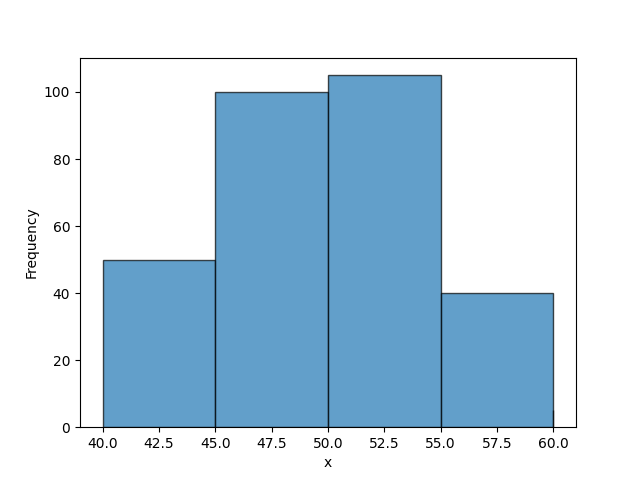
\includegraphics[width = 0.8\linewidth]{../graphics/2_hist.png}
				\caption{Гистограмма}
			\end{center}
		\end{subfigure}

		\begin{subfigure}[htbp!]{0.8\textwidth}
			\begin{center}
				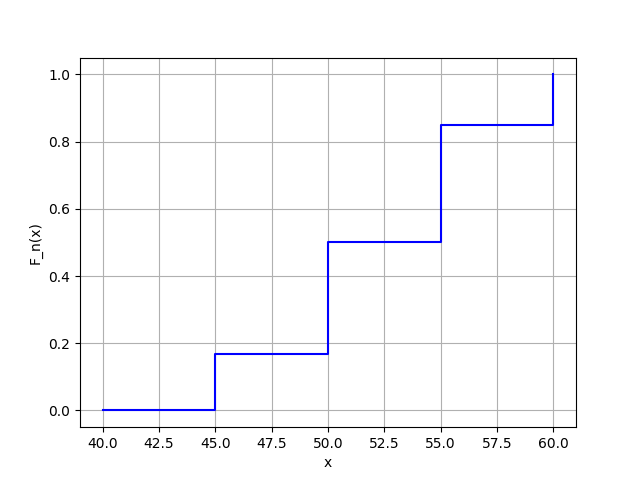
\includegraphics[width = 0.8\linewidth]{../graphics/2_cdf.png}
				\caption{Эмпирическая функция распределения}
			\end{center}
		\end{subfigure}

		\begin{subtable}[htbp!]{0.8\textwidth}
			\centering
			\begin{tabular}{ |c|c|c|c|c|c|c| }
				\hline
				& \( \bar x \) & \( med x \) & \( D(x) \) & \( CV \) & \( A \) & \( E \) \\
				\hline
				Без флактуаций & 49.96 & 50.0 & 22.81 & 0.1 & 0.05 & -0.8 \\
				\hline
				С флактуациями & 780.76 & 1000.0 & 160226.42 & 0.51 & -1.28 & -0.37 \\
				\hline
			\end{tabular}
		\end{subtable}
	\end{figure}

	\begin{figure}
		\begin{subfigure}[htbp!]{0.8\textwidth}
			\begin{center}
				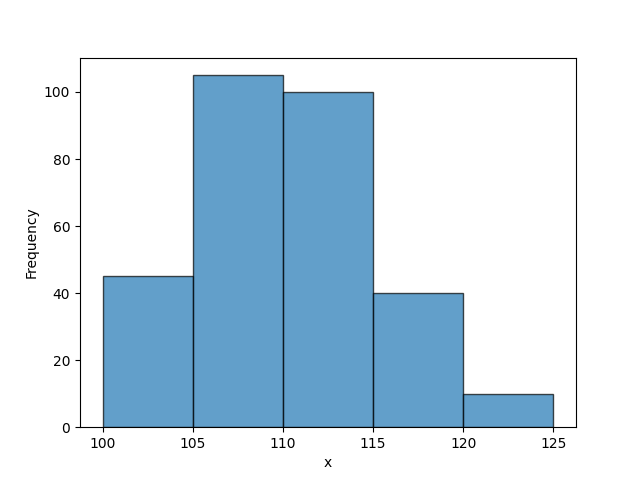
\includegraphics[width = 0.8\linewidth]{../graphics/3_hist.png}
				\caption{Гистограмма}
			\end{center}
		\end{subfigure}

		\begin{subfigure}[htbp!]{0.8\textwidth}
			\begin{center}
				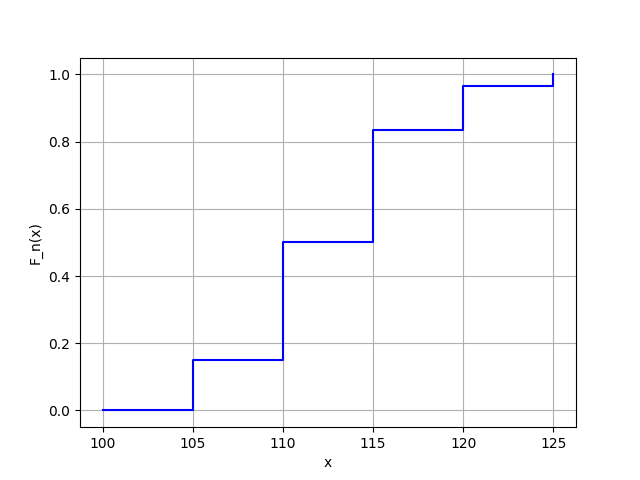
\includegraphics[width = 0.8\linewidth]{../graphics/3_cdf.png}
				\caption{Эмпирическая функция распределения}
			\end{center}
		\end{subfigure}

		\begin{subtable}[htbp!]{0.8\textwidth}
			\centering
			\begin{tabular}{ |c|c|c|c|c|c|c| }
				\hline
				& \( \bar x \) & \( med x \) & \( D(x) \) & \( CV \) & \( A \) & \( E \) \\
				\hline
				Без флактуаций & 110.25 & 110.0 & 25.35 & 0.05 & 0.3 & -0.37 \\
				\hline
				С флактуациями & 794.67 & 1000.0 & 140536.34 & 0.47 & -1.28 & -0.37 \\
				\hline
			\end{tabular}
		\end{subtable}
	\end{figure}

	\begin{figure}
		\begin{subfigure}[htbp!]{0.8\textwidth}
			\begin{center}
				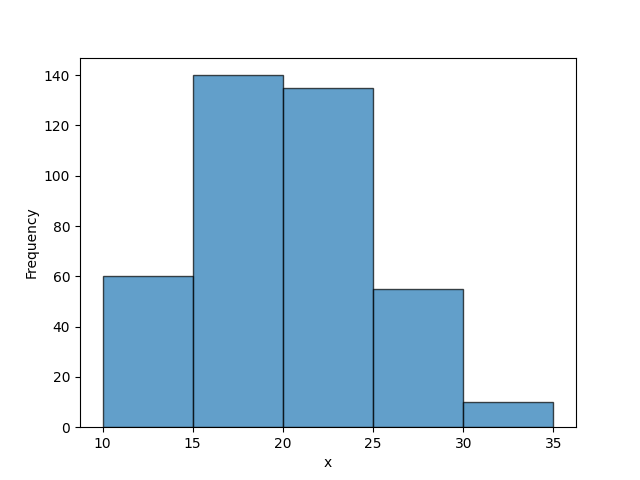
\includegraphics[width = 0.8\linewidth]{../graphics/4_hist.png}
				\caption{Гистограмма}
			\end{center}
		\end{subfigure}

		\begin{subfigure}[htbp!]{0.8\textwidth}
			\begin{center}
				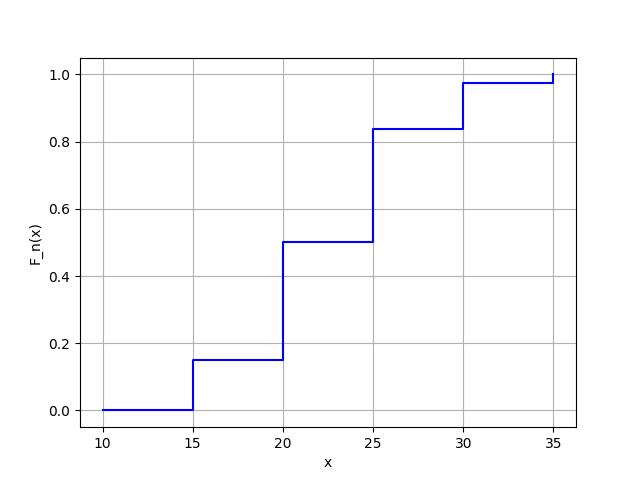
\includegraphics[width = 0.8\linewidth]{../graphics/4_cdf.png}
				\caption{Эмпирическая функция распределения}
			\end{center}
		\end{subfigure}

		\begin{subtable}[htbp!]{0.8\textwidth}
			\centering
			\begin{tabular}{ |c|c|c|c|c|c|c| }
				\hline
				& \( \bar x \) & \( med x \) & \( D(x) \) & \( CV \) & \( A \) & \( E \) \\
				\hline
				Без флактуаций & 110.25 & 110.0 & 25.35 & 0.05 & 0.3 & -0.37 \\
				\hline
				С флактуациями & 794.67 & 1000.0 & 140536.34 & 0.47 & -1.28 & -0.37 \\
				\hline
			\end{tabular}
		\end{subtable}
	\end{figure}

	\begin{figure}
		\begin{subfigure}[htbp!]{0.8\textwidth}
			\begin{center}
				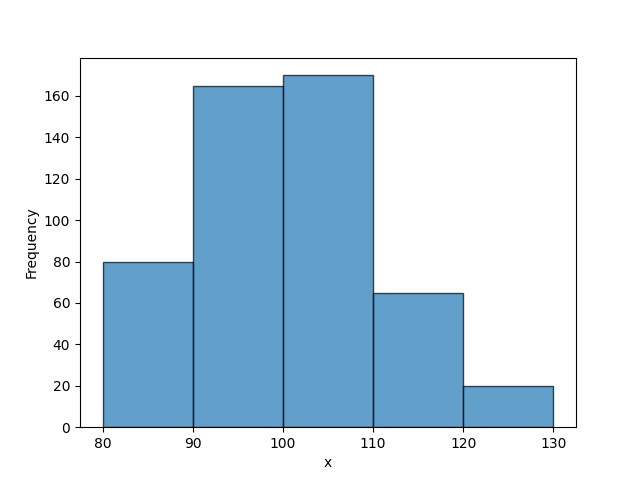
\includegraphics[width = 0.8\linewidth]{../graphics/5_hist.png}
				\caption{Гистограмма}
			\end{center}
		\end{subfigure}

		\begin{subfigure}[htbp!]{0.8\textwidth}
			\begin{center}
				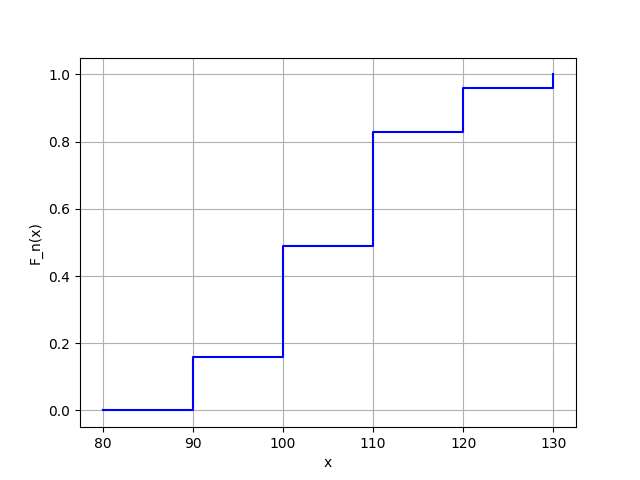
\includegraphics[width = 0.8\linewidth]{../graphics/5_cdf.png}
				\caption{Эмпирическая функция распределения}
			\end{center}
		\end{subfigure}

		\begin{subtable}[htbp!]{0.8\textwidth}
			\centering
			\begin{tabular}{ |c|c|c|c|c|c|c| }
				\hline
				& \( \bar x \) & \( med x \) & \( D(x) \) & \( CV \) & \( A \) & \( E \) \\
				\hline
				Без флактуаций & 100.6 & 105.0 & 106.64 & 0.1 & 0.3 & -0.39 \\
				\hline
				С флактуациями & 700.2 & 1000.0 & 179795.63 & 0.61 & -0.71 & -1.5 \\
				\hline
			\end{tabular}
		\end{subtable}
	\end{figure}

	\begin{figure}
		\begin{subfigure}[htbp!]{0.8\textwidth}
			\begin{center}
				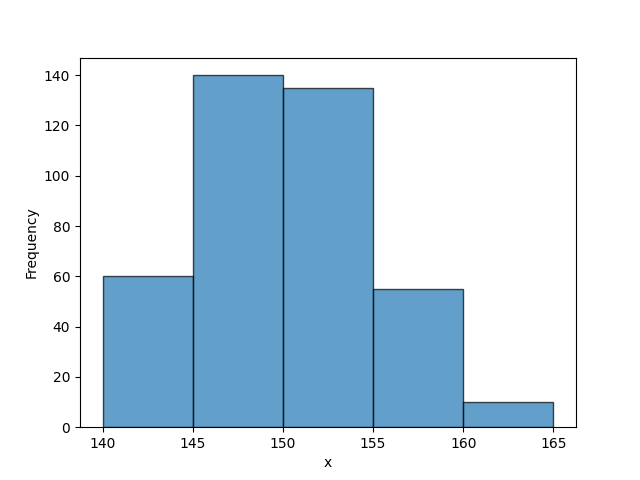
\includegraphics[width = 0.8\linewidth]{../graphics/6_hist.png}
				\caption{Гистограмма}
			\end{center}
		\end{subfigure}

		\begin{subfigure}[htbp!]{0.8\textwidth}
			\begin{center}
				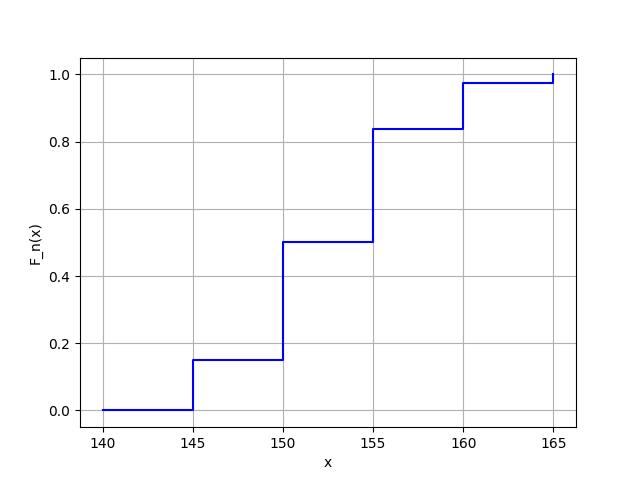
\includegraphics[width = 0.8\linewidth]{../graphics/6_cdf.png}
				\caption{Эмпирическая функция распределения}
			\end{center}
		\end{subfigure}

		\begin{subtable}[htbp!]{0.8\textwidth}
			\centering
			\begin{tabular}{ |c|c|c|c|c|c|c| }
				\hline
				& \( \bar x \) & \( med x \) & \( D(x) \) & \( CV \) & \( A \) & \( E \) \\
				\hline
				Без флактуаций & 150.19 & 150.0 & 24.34 & 0.03 & 0.25 & -0.44 \\
				\hline
				С флактуациями & 757.2 & 1000.0 & 147390.89 & 0.51 & -0.95 & -1.1 \\
				\hline
			\end{tabular}
		\end{subtable}
	\end{figure}

	\begin{figure}
		\begin{subfigure}[htbp!]{0.8\textwidth}
			\begin{center}
				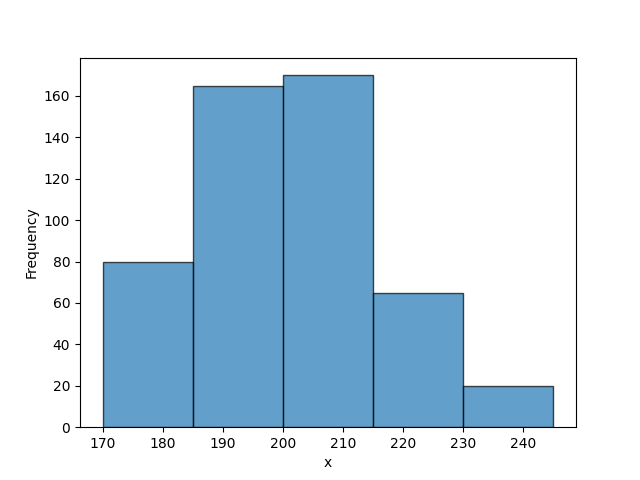
\includegraphics[width = 0.8\linewidth]{../graphics/7_hist.png}
				\caption{Гистограмма}
			\end{center}
		\end{subfigure}

		\begin{subfigure}[htbp!]{0.8\textwidth}
			\begin{center}
				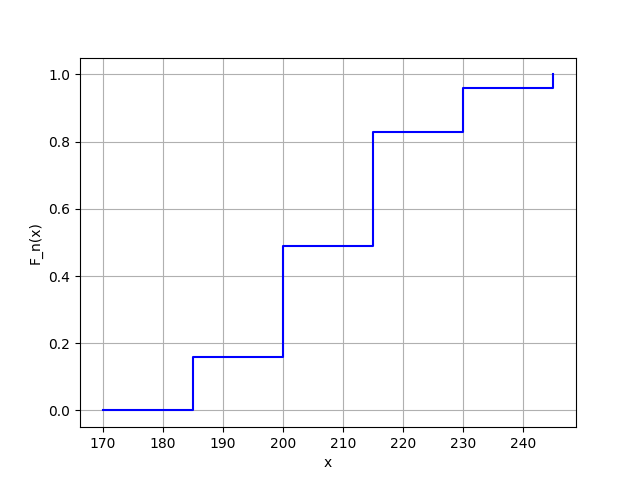
\includegraphics[width = 0.8\linewidth]{../graphics/7_cdf.png}
				\caption{Эмпирическая функция распределения}
			\end{center}
		\end{subfigure}

		\begin{subtable}[htbp!]{0.8\textwidth}
			\centering
			\begin{tabular}{ |c|c|c|c|c|c|c| }
				\hline
				& \( \bar x \) & \( med x \) & \( D(x) \) & \( CV \) & \( A \) & \( E \) \\
				\hline
				Без флактуаций & 200.9 & 207.5 & 239.94 & 0.08 & 0.3 & -0.39 \\
				\hline
				С флактуациями & 733.63 & 1000.0 & 141982.38 & 0.51 & -0.71 & -1.49 \\
				\hline
			\end{tabular}
		\end{subtable}
	\end{figure}

	\begin{figure}
		\begin{subfigure}[htbp!]{0.8\textwidth}
			\begin{center}
				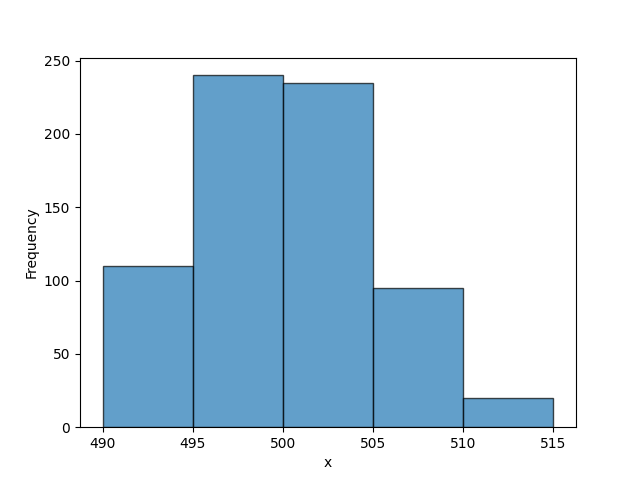
\includegraphics[width = 0.8\linewidth]{../graphics/8_hist.png}
				\caption{Гистограмма}
			\end{center}
		\end{subfigure}

		\begin{subfigure}[htbp!]{0.8\textwidth}
			\begin{center}
				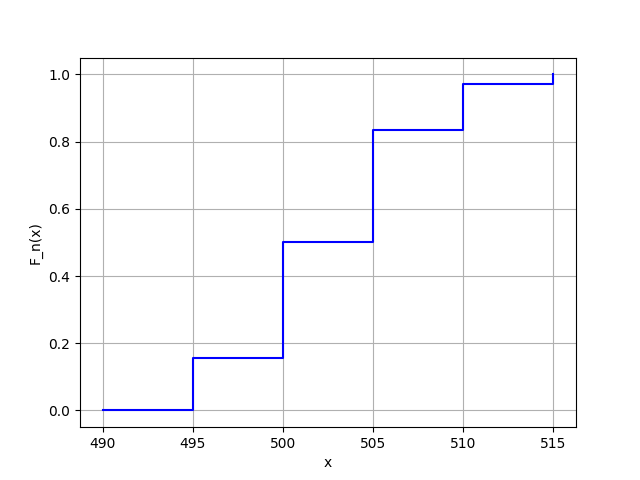
\includegraphics[width = 0.8\linewidth]{../graphics/8_cdf.png}
				\caption{Эмпирическая функция распределения}
			\end{center}
		\end{subfigure}

		\begin{subtable}[htbp!]{0.8\textwidth}
			\centering
			\begin{tabular}{ |c|c|c|c|c|c|c| }
				\hline
				& \( \bar x \) & \( med x \) & \( D(x) \) & \( CV \) & \( A \) & \( E \) \\
				\hline
				Без флактуаций & 500.18 & 500.0 & 25.15 & 0.01 & 0.26 & -0.43 \\
				\hline
				С флактуациями & 794.19 & 1000.0 & 60520.74 & 0.31 & -0.36 & -1.87 \\
				\hline
			\end{tabular}
		\end{subtable}
	\end{figure}

	\begin{figure}
		\begin{subfigure}[htbp!]{0.8\textwidth}
			\begin{center}
				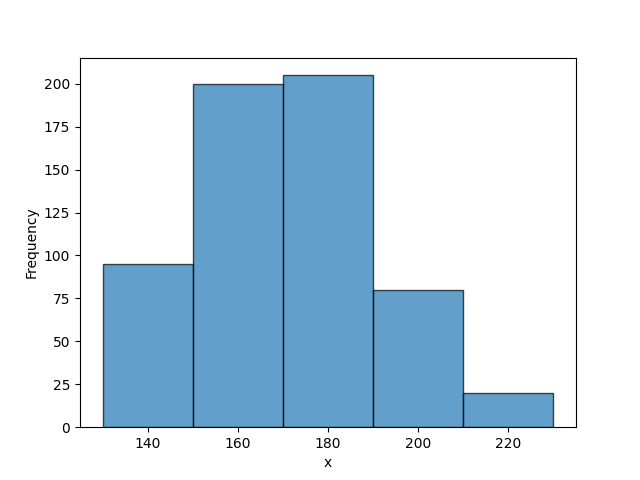
\includegraphics[width = 0.8\linewidth]{../graphics/9_hist.png}
				\caption{Гистограмма}
			\end{center}
		\end{subfigure}

		\begin{subfigure}[htbp!]{0.8\textwidth}
			\begin{center}
				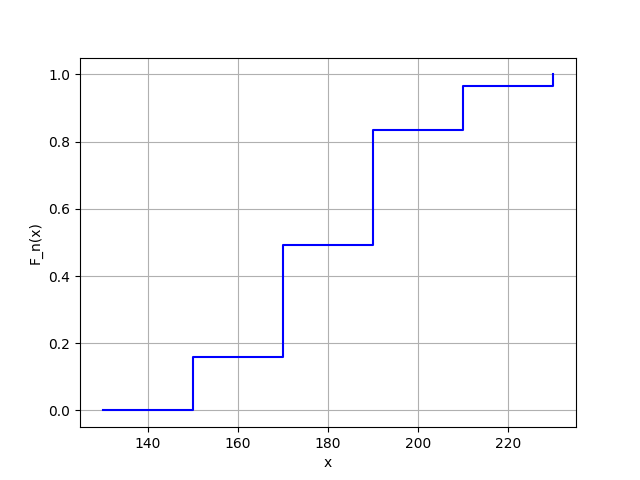
\includegraphics[width = 0.8\linewidth]{../graphics/9_cdf.png}
				\caption{Эмпирическая функция распределения}
			\end{center}
		\end{subfigure}

		\begin{subtable}[htbp!]{0.8\textwidth}
			\centering
			\begin{tabular}{ |c|c|c|c|c|c|c| }
				\hline
				& \( \bar x \) & \( med x \) & \( D(x) \) & \( CV \) & \( A \) & \( E \) \\
				\hline
				Без флактуаций & 171.0 & 180.0 & 412.33 & 0.12 & 0.27 & -0.41 \\
				\hline
				С флактуациями & 689.12 & 1000.0 & 161226.73 & 0.58 & -0.52 & -1.73 \\
				\hline
			\end{tabular}
		\end{subtable}
	\end{figure}

	\begin{figure}
		\begin{subfigure}[htbp!]{0.8\textwidth}
			\begin{center}
				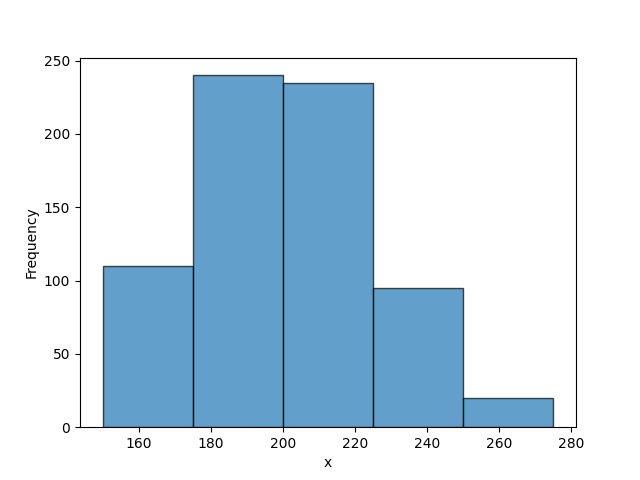
\includegraphics[width = 0.8\linewidth]{../graphics/10_hist.png}
				\caption{Гистограмма}
			\end{center}
		\end{subfigure}

		\begin{subfigure}[htbp!]{0.8\textwidth}
			\begin{center}
				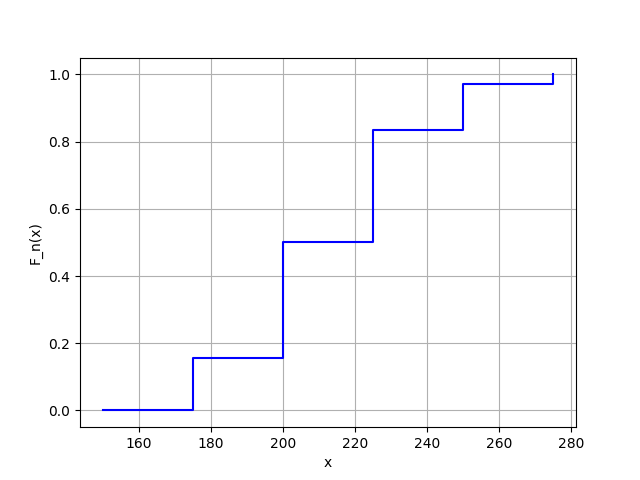
\includegraphics[width = 0.8\linewidth]{../graphics/10_cdf.png}
				\caption{Эмпирическая функция распределения}
			\end{center}
		\end{subfigure}

		\begin{subtable}[htbp!]{0.8\textwidth}
			\centering
			\begin{tabular}{ |c|c|c|c|c|c|c| }
				\hline
				& \( \bar x \) & \( med x \) & \( D(x) \) & \( CV \) & \( A \) & \( E \) \\
				\hline
				Без флактуаций & 200.89 & 200.0 & 628.67 & 0.12 & 0.26 & -0.43 \\
				\hline
				С флактуациями & 670.96 & 1000.0 & 154930.34 & 0.59 & -0.36 & -1.86 \\
				\hline
			\end{tabular}
		\end{subtable}
	\end{figure}

	\newpage

	\section{Выводы}

	В ходе проведения лабораторной работы вы обнаружите, что выборочные значения, такие как среднее значение, дисперсия, медиана, коэффициент вариации, коэффициент асимметрии и эксцесс, дают важное понимание свойств вашего распределения данных. Гистограмма и график эмпирической функции распределения Fn(x) также являются полезными инструментами для визуализации распределения ваших данных.

	Добавление искусственной флуктуации к данным, особенно большой (порядка 1000), приводит к значительным изменениям во всех ваших статистических показателях. Среднее значение и дисперсия, вероятно, увеличатся значительно, так как они чувствительны к отклонениям и изменениям в данных. Коэффициент вариации также увеличится, отражая увеличившуюся вариативность данных. Коэффициенты асимметрии и эксцесса также могут значительно измениться, изменяя форму распределения.

	Эти изменения объясняются тем, что введенная флуктуация является значительной по отношению к текущим данным, что приводит к резкому увеличению разброса данных. Это подчеркивает важность устойчивых и высококачественных данных при проведении статистического анализа, поскольку аномальные значения могут сильно искажать наши оценки и выводы.
\end{document}
